\chapter{نتایج و تحلیل‌ها}

\section{ارزیابی بر روی مجموعه‌داده \lr{CIFAR-10}}

به منظور ارزیابی عملکرد مدل پیشنهادی، دو پیکربندی مجزا مورد مقایسه قرار گرفتند:  
\begin{enumerate}
	\item مدل مبنا: \lr{Tiny Swin Transformer} به عنوان معماری اصلی بدون اعمال تغییرات.
	\item مدل پیشنهادی: \lr{Tensorized Swin Transformer} که در آن لایه‌های \lr{Patch Embedding}، \lr{W-MSA} و \lr{Patch Merging} به کمک تکنیک فشرده‌سازی تانسوری بازطراحی شده‌اند.
\end{enumerate}

\subsection{خلاصه نتایج کمی}

جدول \ref{tab:cifar10_summary_tensor} نتایج کمی این دو مدل را در شاخص‌های دقت \lr{Top-1} و \lr{Top-5} برای داده‌های آموزش و آزمون نشان می‌دهد.  
در این جدول ترتیب ستون‌ها به‌گونه‌ای تنظیم شده است که مقایسه میان عملکرد آموزشی و آزمونی به‌صورت هم‌زمان و از راست به چپ قابل مشاهده باشد.

\begin{table}[ht]
	\centering
	\caption{مقایسه عملکرد مدل اصلی و مدل پیشنهادی بر روی مجموعه‌داده \lr{CIFAR-10} بر حسب دقت‌های \lr{Top-1} و \lr{Top-5}.}
	\label{tab:cifar10_summary_tensor}
	\begin{tabular}{ccccccl}
		\hline
		\multicolumn{2}{c}{داده آزمون} & \multicolumn{2}{c}{داده آموزش} & \multirow{2}{*}{\#پارامترها} & \multirow{2}{*}{مدل} \\
		\cline{1-4}
		Top-5 & Top-1 & Top-5 & Top-1 &  &  \\
		\hline
		\lr{96.45\%} & \lr{80.92\%} & \lr{99.97\%} & \lr{97.48\%} & \lr{27,528,690} & \lr{Tiny Swin} \\
		\lr{99.21\%} & \lr{81.80\%} & \lr{98.97\%} & \lr{80.30\%} & \lr{1,368,626} & \lr{Tensorized Swin} \\
		\hline
	\end{tabular}
\end{table}

\subsection{تحلیل نتایج}

مطابق داده‌های جدول \ref{tab:cifar10_summary_tensor}، مدل پیشنهادی با وجود کاهش چشم‌گیر تعداد پارامترها (از حدود \lr{27.5M} به حدود \lr{1.37M}، معادل کاهش \lr{95\%})، توانسته است دقت آزمون را حفظ یا حتی اندکی بهبود بخشد.  
در شاخص \lr{Top-1}، دقت مدل اصلی در داده آزمون برابر \lr{80.92\%} بوده که در مدل تانسوری به \lr{81.80\%} رسیده است.  
همچنین در شاخص \lr{Top-5}، بهبود محسوس‌تری مشاهده می‌شود؛ به‌طوری که مقدار دقت از \lr{96.45\%} به \lr{99.21\%} افزایش یافته است.  

از سوی دیگر، بررسی شکاف آموزش–آزمون نشان می‌دهد که مدل اصلی با اختلاف \lr{16.56} واحد درصد بین دقت آموزشی (\lr{97.48\%}) و آزمونی (\lr{80.92\%}) دچار بیش‌برازش (\lr{Overfitting}) بوده است.  
در حالی که مدل تانسوری نه تنها چنین شکافی ندارد، بلکه دقت آزمونی آن اندکی از دقت آموزشی بیشتر است (اختلاف \lr{-1.5} واحد درصد).  
این امر بیانگر وجود نوعی منظم‌سازی ذاتی (\lr{Implicit Regularization}) ناشی از فشرده‌سازی تانسوری و اعمال قیود کم‌مرتبه (\lr{Low-Rank Constraints}) است.  

بهبود محسوس در \lr{Top-5} نیز حاکی از آن است که مدل پیشنهادی فضای ویژگی غنی‌تری ایجاد کرده که امکان پوشش کلاس‌های صحیح در میان پنج پیش‌بینی برتر را افزایش داده و در نتیجه اطمینان کلی تصمیم‌گیری مدل را ارتقاء داده است.

\subsection{نمایش روند آموزش}

برای درک بهتر فرایند همگرایی، روند تغییرات دقت \lr{Top-1} در طول آموزش برای هر دو مدل در شکل‌های \ref{fig:cifar10_swin_original} و \ref{fig:cifar10_tensorized} نمایش داده شده است.  
این نمودارها نشان می‌دهند که مدل اصلی به سرعت به دقت بالایی در داده آموزشی می‌رسد ولی در داده آزمون افت می‌کند، در حالی که مدل تانسوری با روندی یکنواخت‌تر و پایدارتر به دقت نهایی می‌رسد.

\begin{figure}[ht]
	\centering
	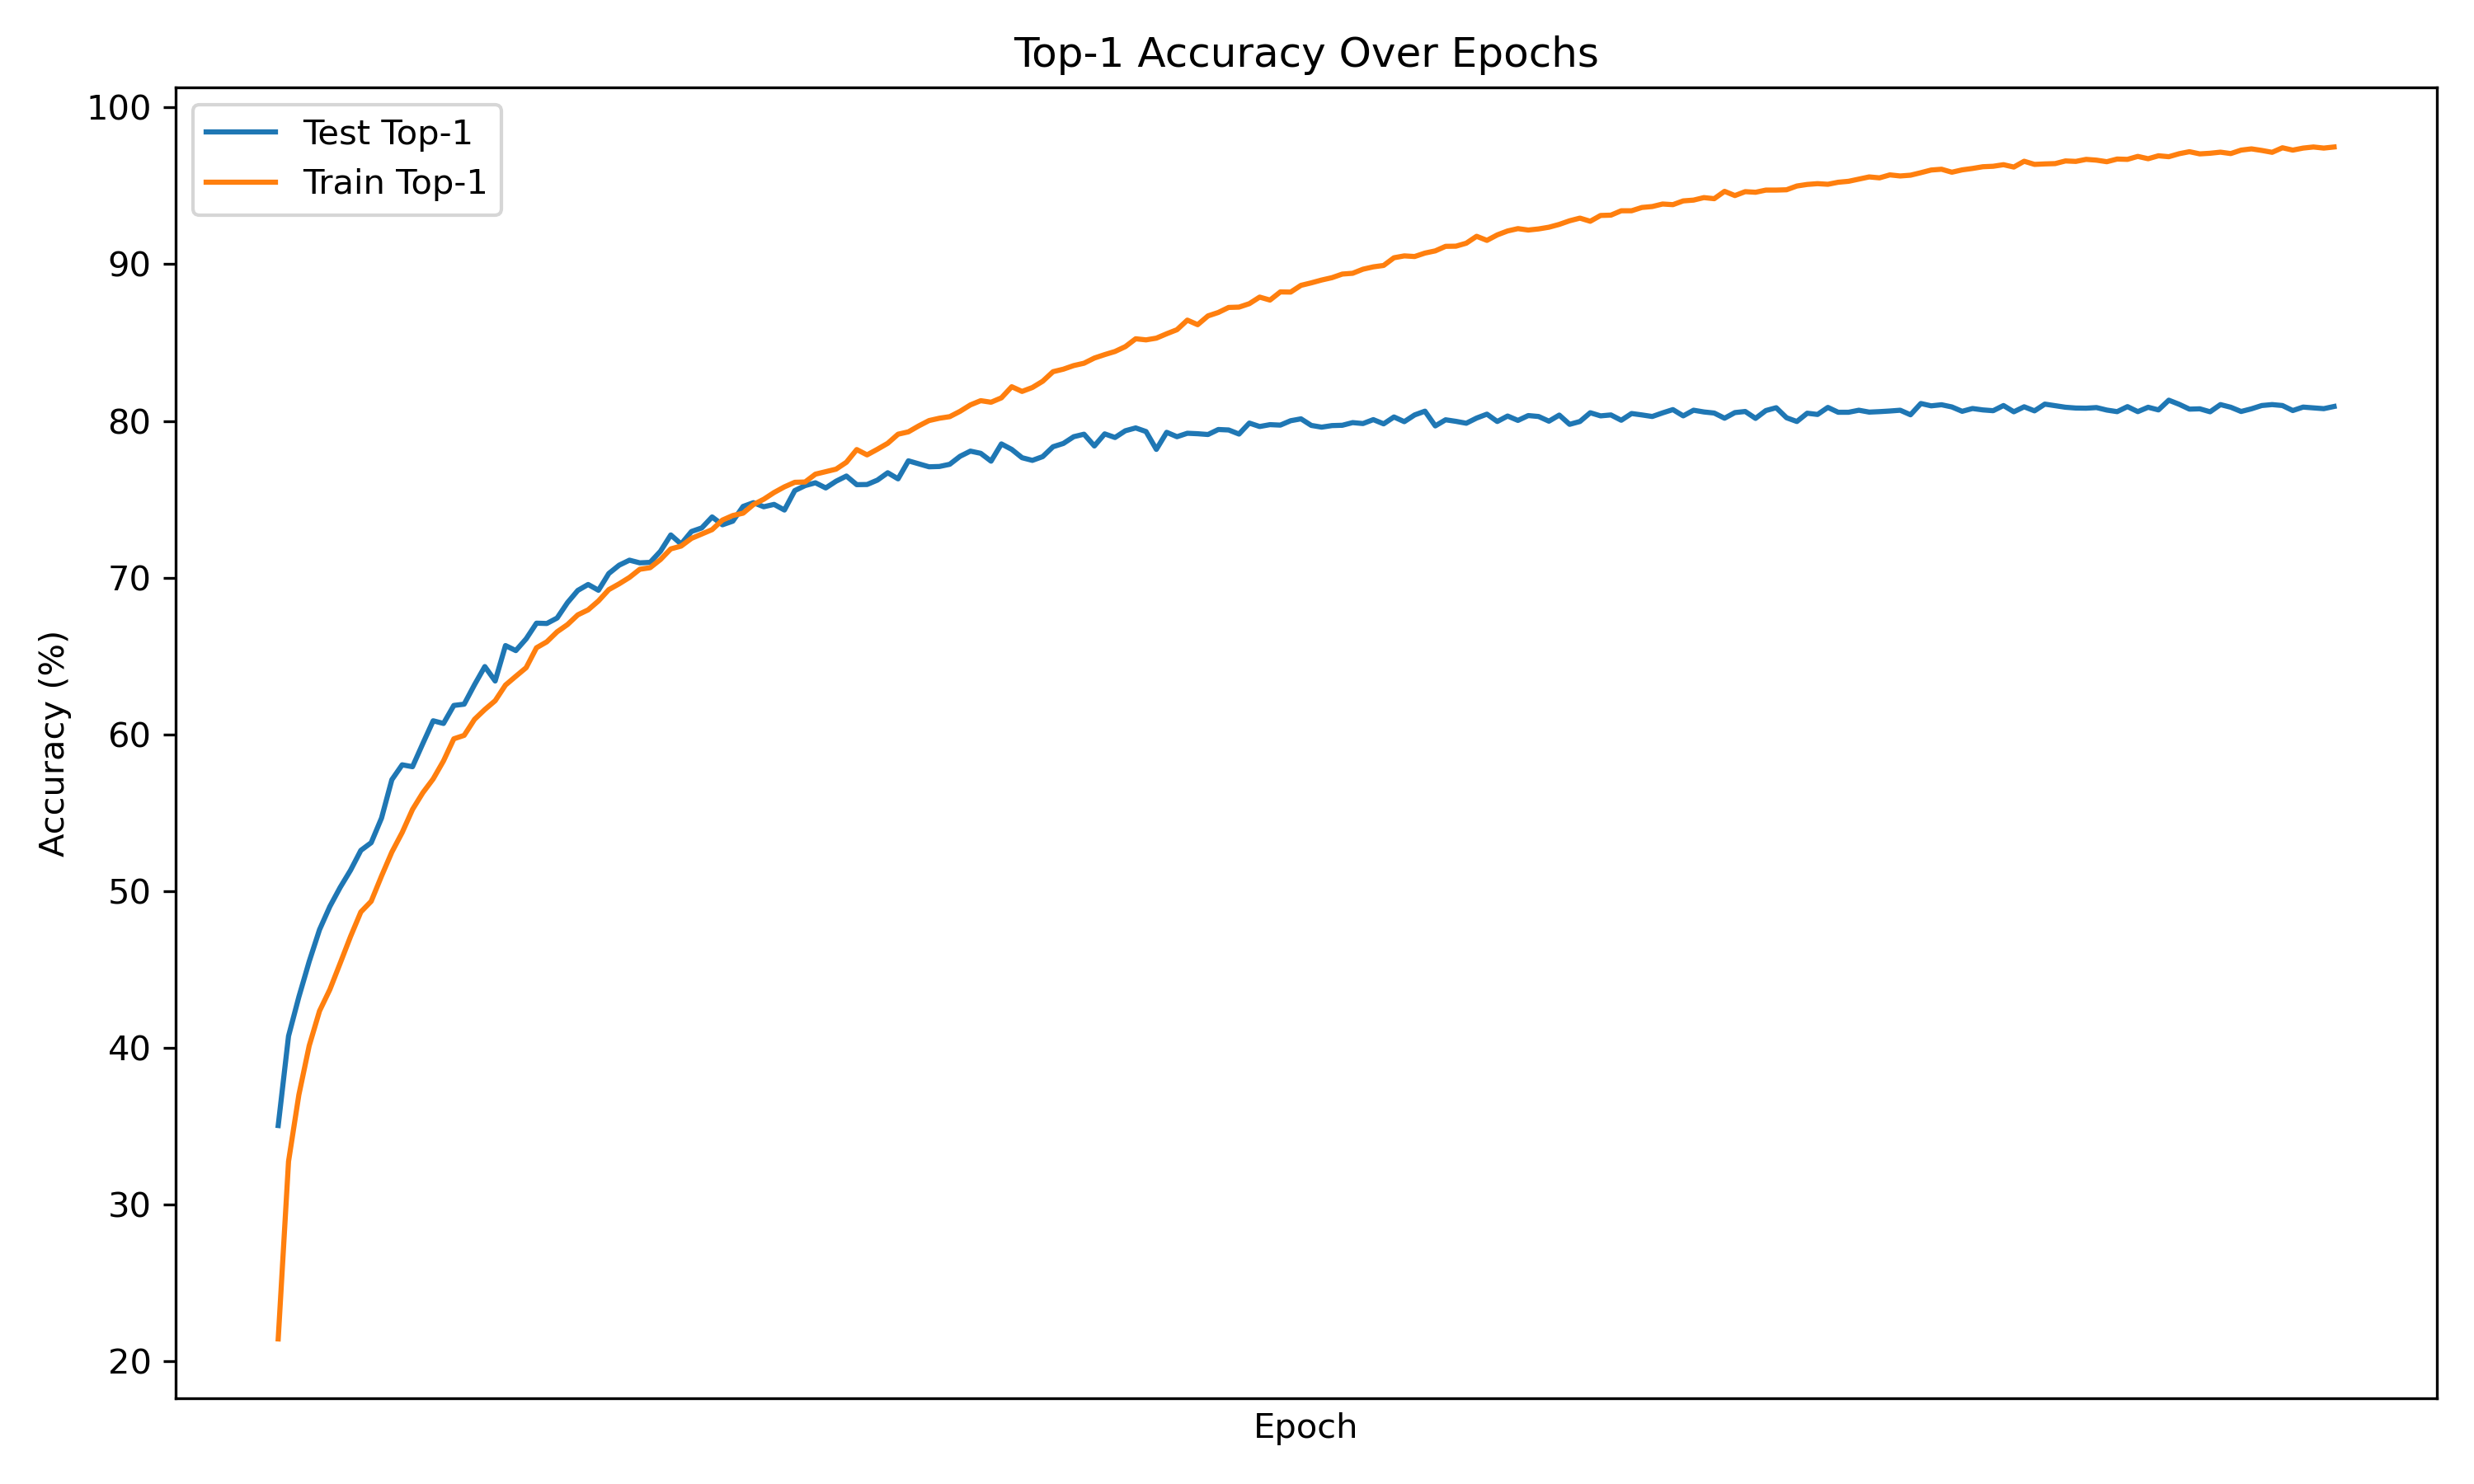
\includegraphics[width=0.85\textwidth]{transformer_images/results/cifar10_swin_original.png}
	\caption{روند تغییرات دقت \lr{Top-1} مدل اصلی \lr{Swin-Tiny} بر روی مجموعه‌داده \lr{CIFAR-10}.}
	\label{fig:cifar10_swin_original}
\end{figure}

\begin{figure}[ht]
	\centering
	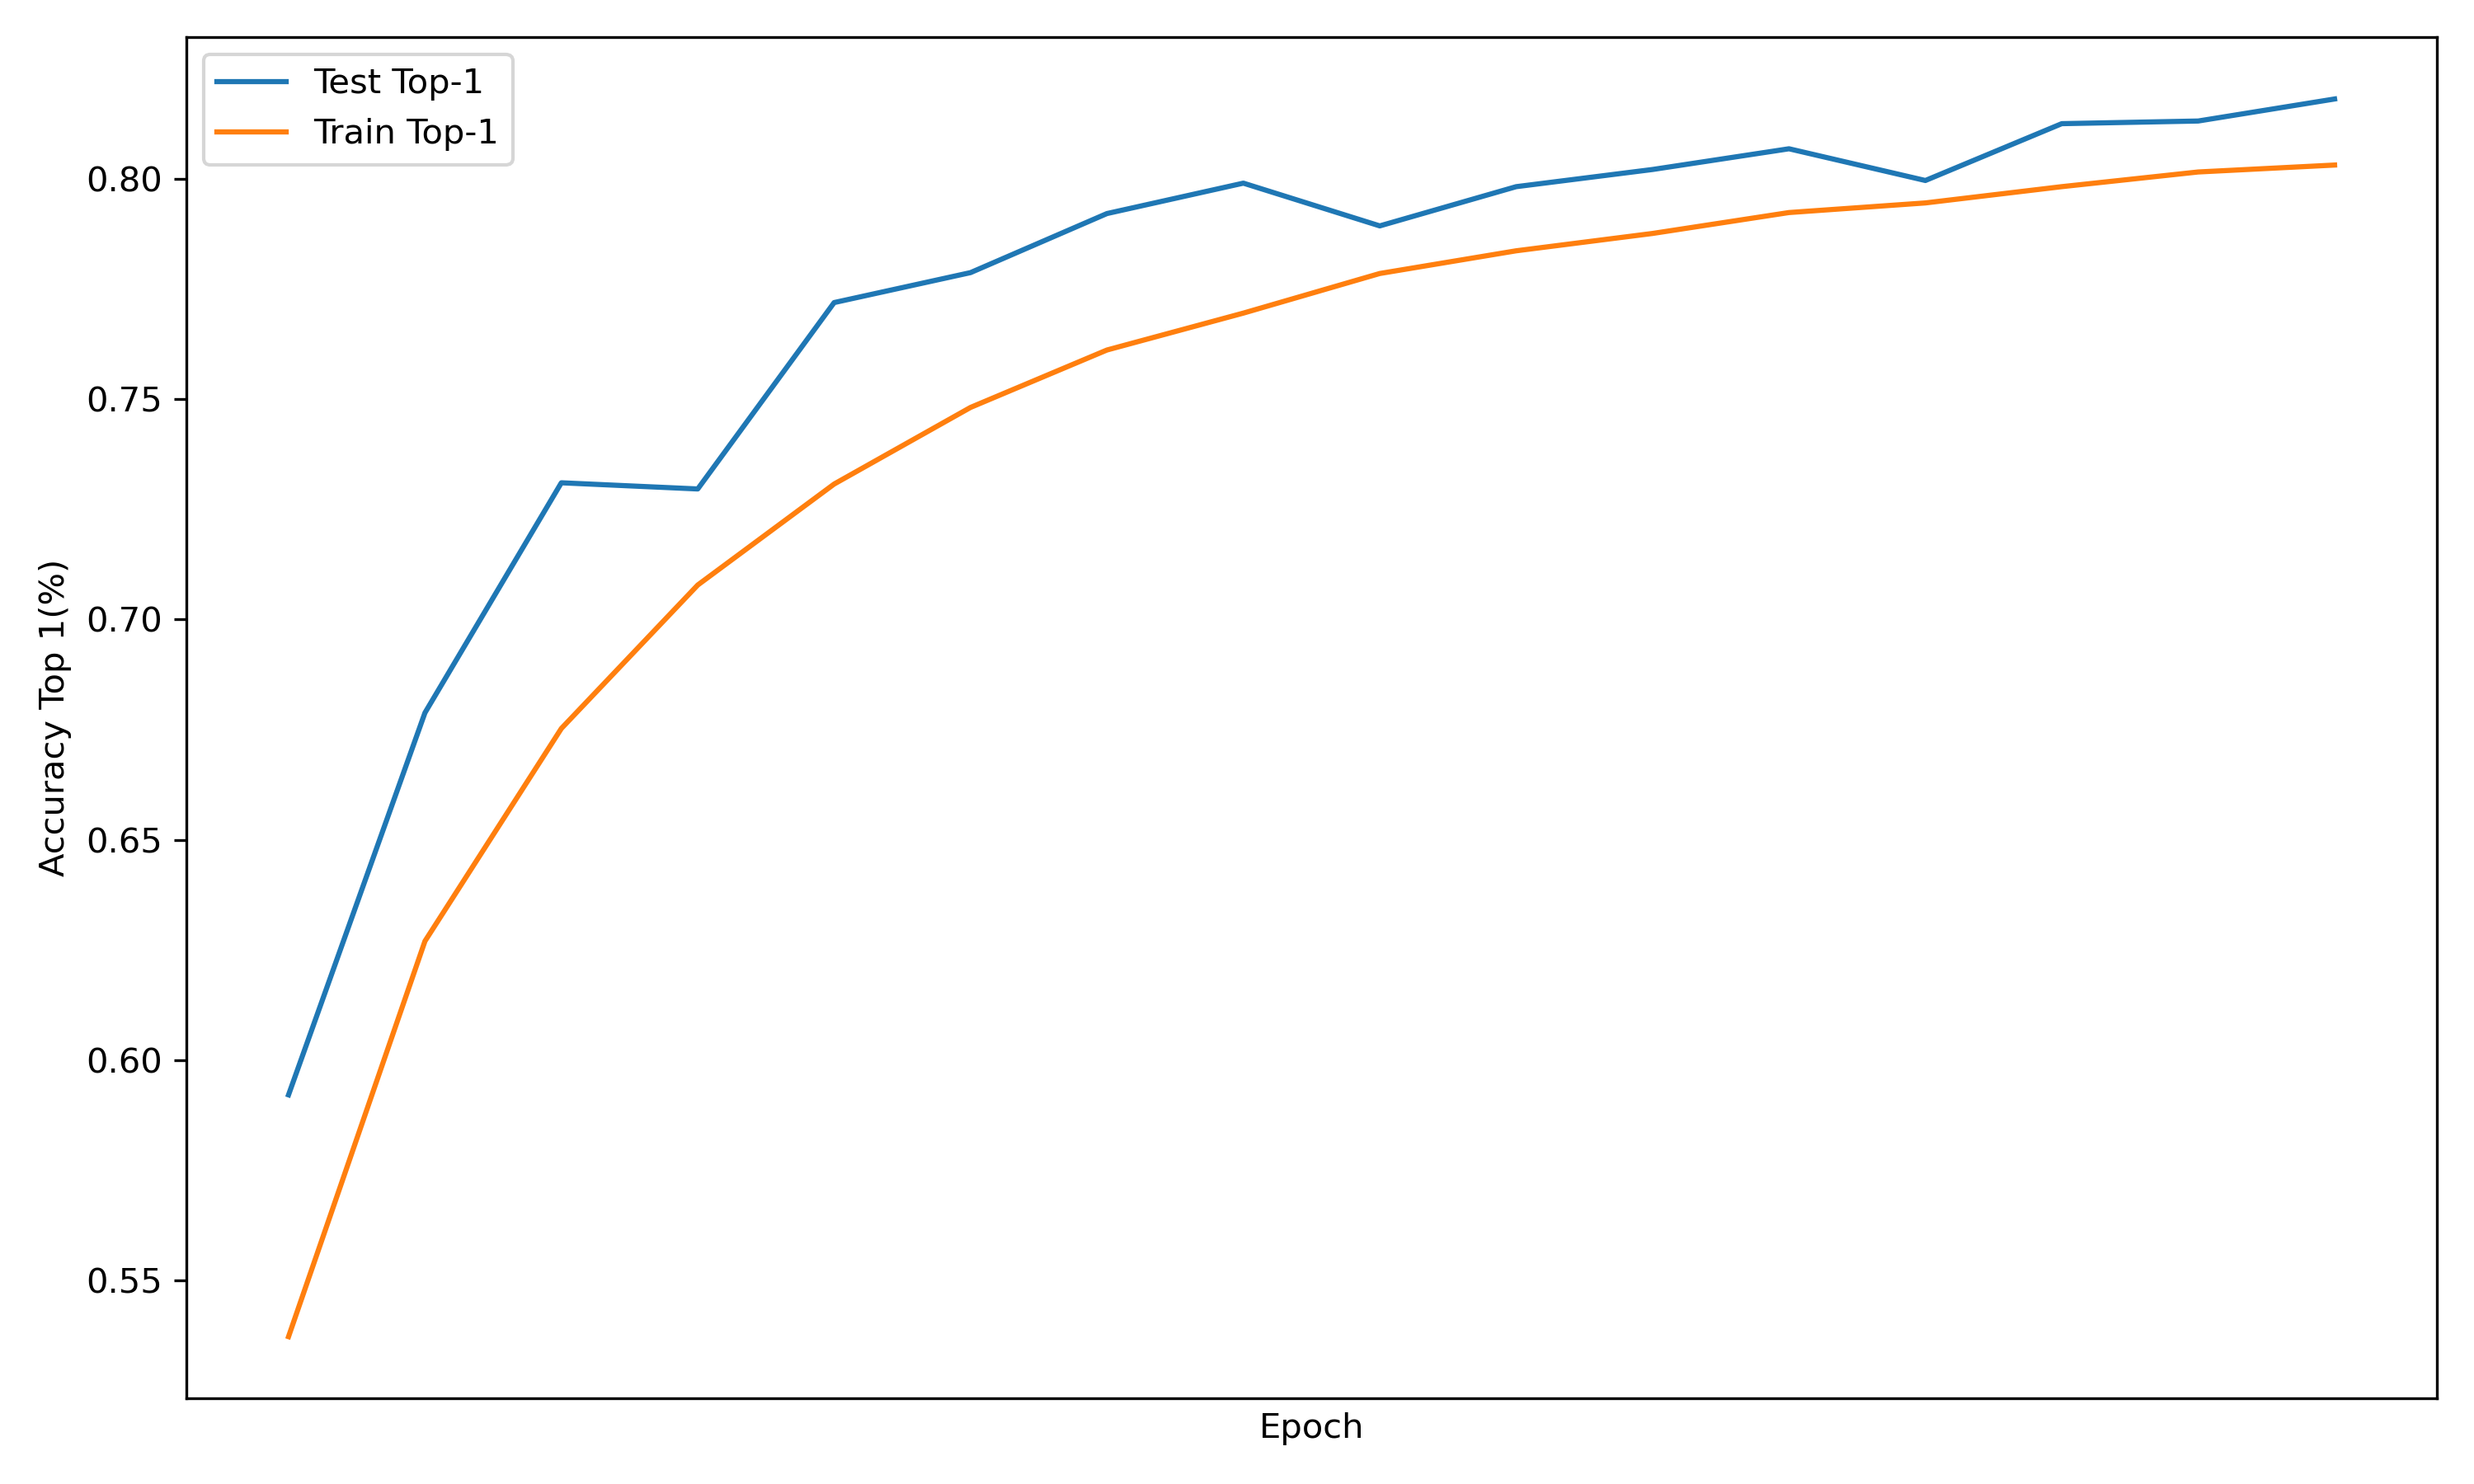
\includegraphics[width=0.85\textwidth]{transformer_images/results/cifar10_tensorized.png}
	\caption{روند تغییرات دقت \lr{Top-1} مدل پیشنهادی \lr{Tensorized Swin} بر روی مجموعه‌داده \lr{CIFAR-10}.}
	\label{fig:cifar10_tensorized}
\end{figure}

\subsection{جمع‌بندی}

به‌طور کلی، نتایج به‌دست‌آمده نشان می‌دهد که استفاده از ساختار تانسوری در بخش‌های کلیدی مدل، علاوه بر کاهش چشم‌گیر پیچیدگی محاسباتی و نیاز حافظه، باعث بهبود تعمیم‌پذیری و کاهش بیش‌برازش نیز می‌شود.  
این امر اهمیت به‌کارگیری روش‌های فشرده‌سازی ساختاریافته را در طراحی مدل‌های کارا برای کاربردهای کم‌منبع تأیید می‌کند.







\section{نتایج بر روی دیتاست \lr{MNIST}}

برای ارزیابی عملکرد مدل پیشنهادی بر روی داده‌های ساده‌تر و با ابعاد کوچک‌تر، آزمایش‌ها بر روی دیتاست \lr{MNIST} نیز انجام شده است. در این ارزیابی دو پیکربندی زیر مقایسه شده‌اند:
\begin{enumerate}
	\item \textbf{مدل اصلی} (\lr{Tiny Swin Transformer})
	\item \textbf{مدل پیشنهادی تانسوری} (\lr{Tensorized Swin Transformer})
\end{enumerate}

\subsection{خلاصه‌ی نتایج کمی}

\begin{table}[ht]
	\centering
	\caption{مقایسه‌ی عملکرد مدل اصلی و مدل تانسوری بر روی \lr{MNIST} (فقط Top-1 و Top-5).}
	\label{tab:mnist_summary_tensor}
	\begin{tabular}{ccccccl} % ستون‌ها به صورت معکوس برای نمایش پایان‌نامه‌ای
		\hline
		\multicolumn{2}{c}{تست} & \multicolumn{2}{c}{آموزش} & \multirow{2}{*}{\#پارامترها} & \multirow{2}{*}{مدل} \\
		\cline{1-4}
		Top-5 & Top-1 & Top-5 & Top-1 &  &  \\
		\hline
		\lr{99.9\%} & \lr{97.0\%} & \lr{99.9\%} & \lr{95.8\%} & \lr{27,528,690} & \lr{Tiny Swin} \\
		\lr{100\%} & \lr{98.9\%} & \lr{99.9\%} & \lr{97.3\%} & \lr{1,368,626} & \lr{Tensorized Swin} \\
		\hline
	\end{tabular}
\end{table}

\subsection{نمایش روند آموزش}

شکل‌های \ref{fig:mnist_swin_original} و \ref{fig:mnist_tensorized} روند تغییرات دقت \lr{Top-1} را برای مدل اصلی و مدل تانسوری بر روی مجموعه‌داده‌ی \lr{MNIST} نشان می‌دهند. هر دو مدل به سرعت به دقت بسیار بالا رسیده‌اند، اما مدل تانسوری با وجود تعداد پارامترهای بسیار کمتر، دقت نهایی بالاتری در داده‌های آزمون کسب کرده است.

\begin{figure}[ht]
	\centering
	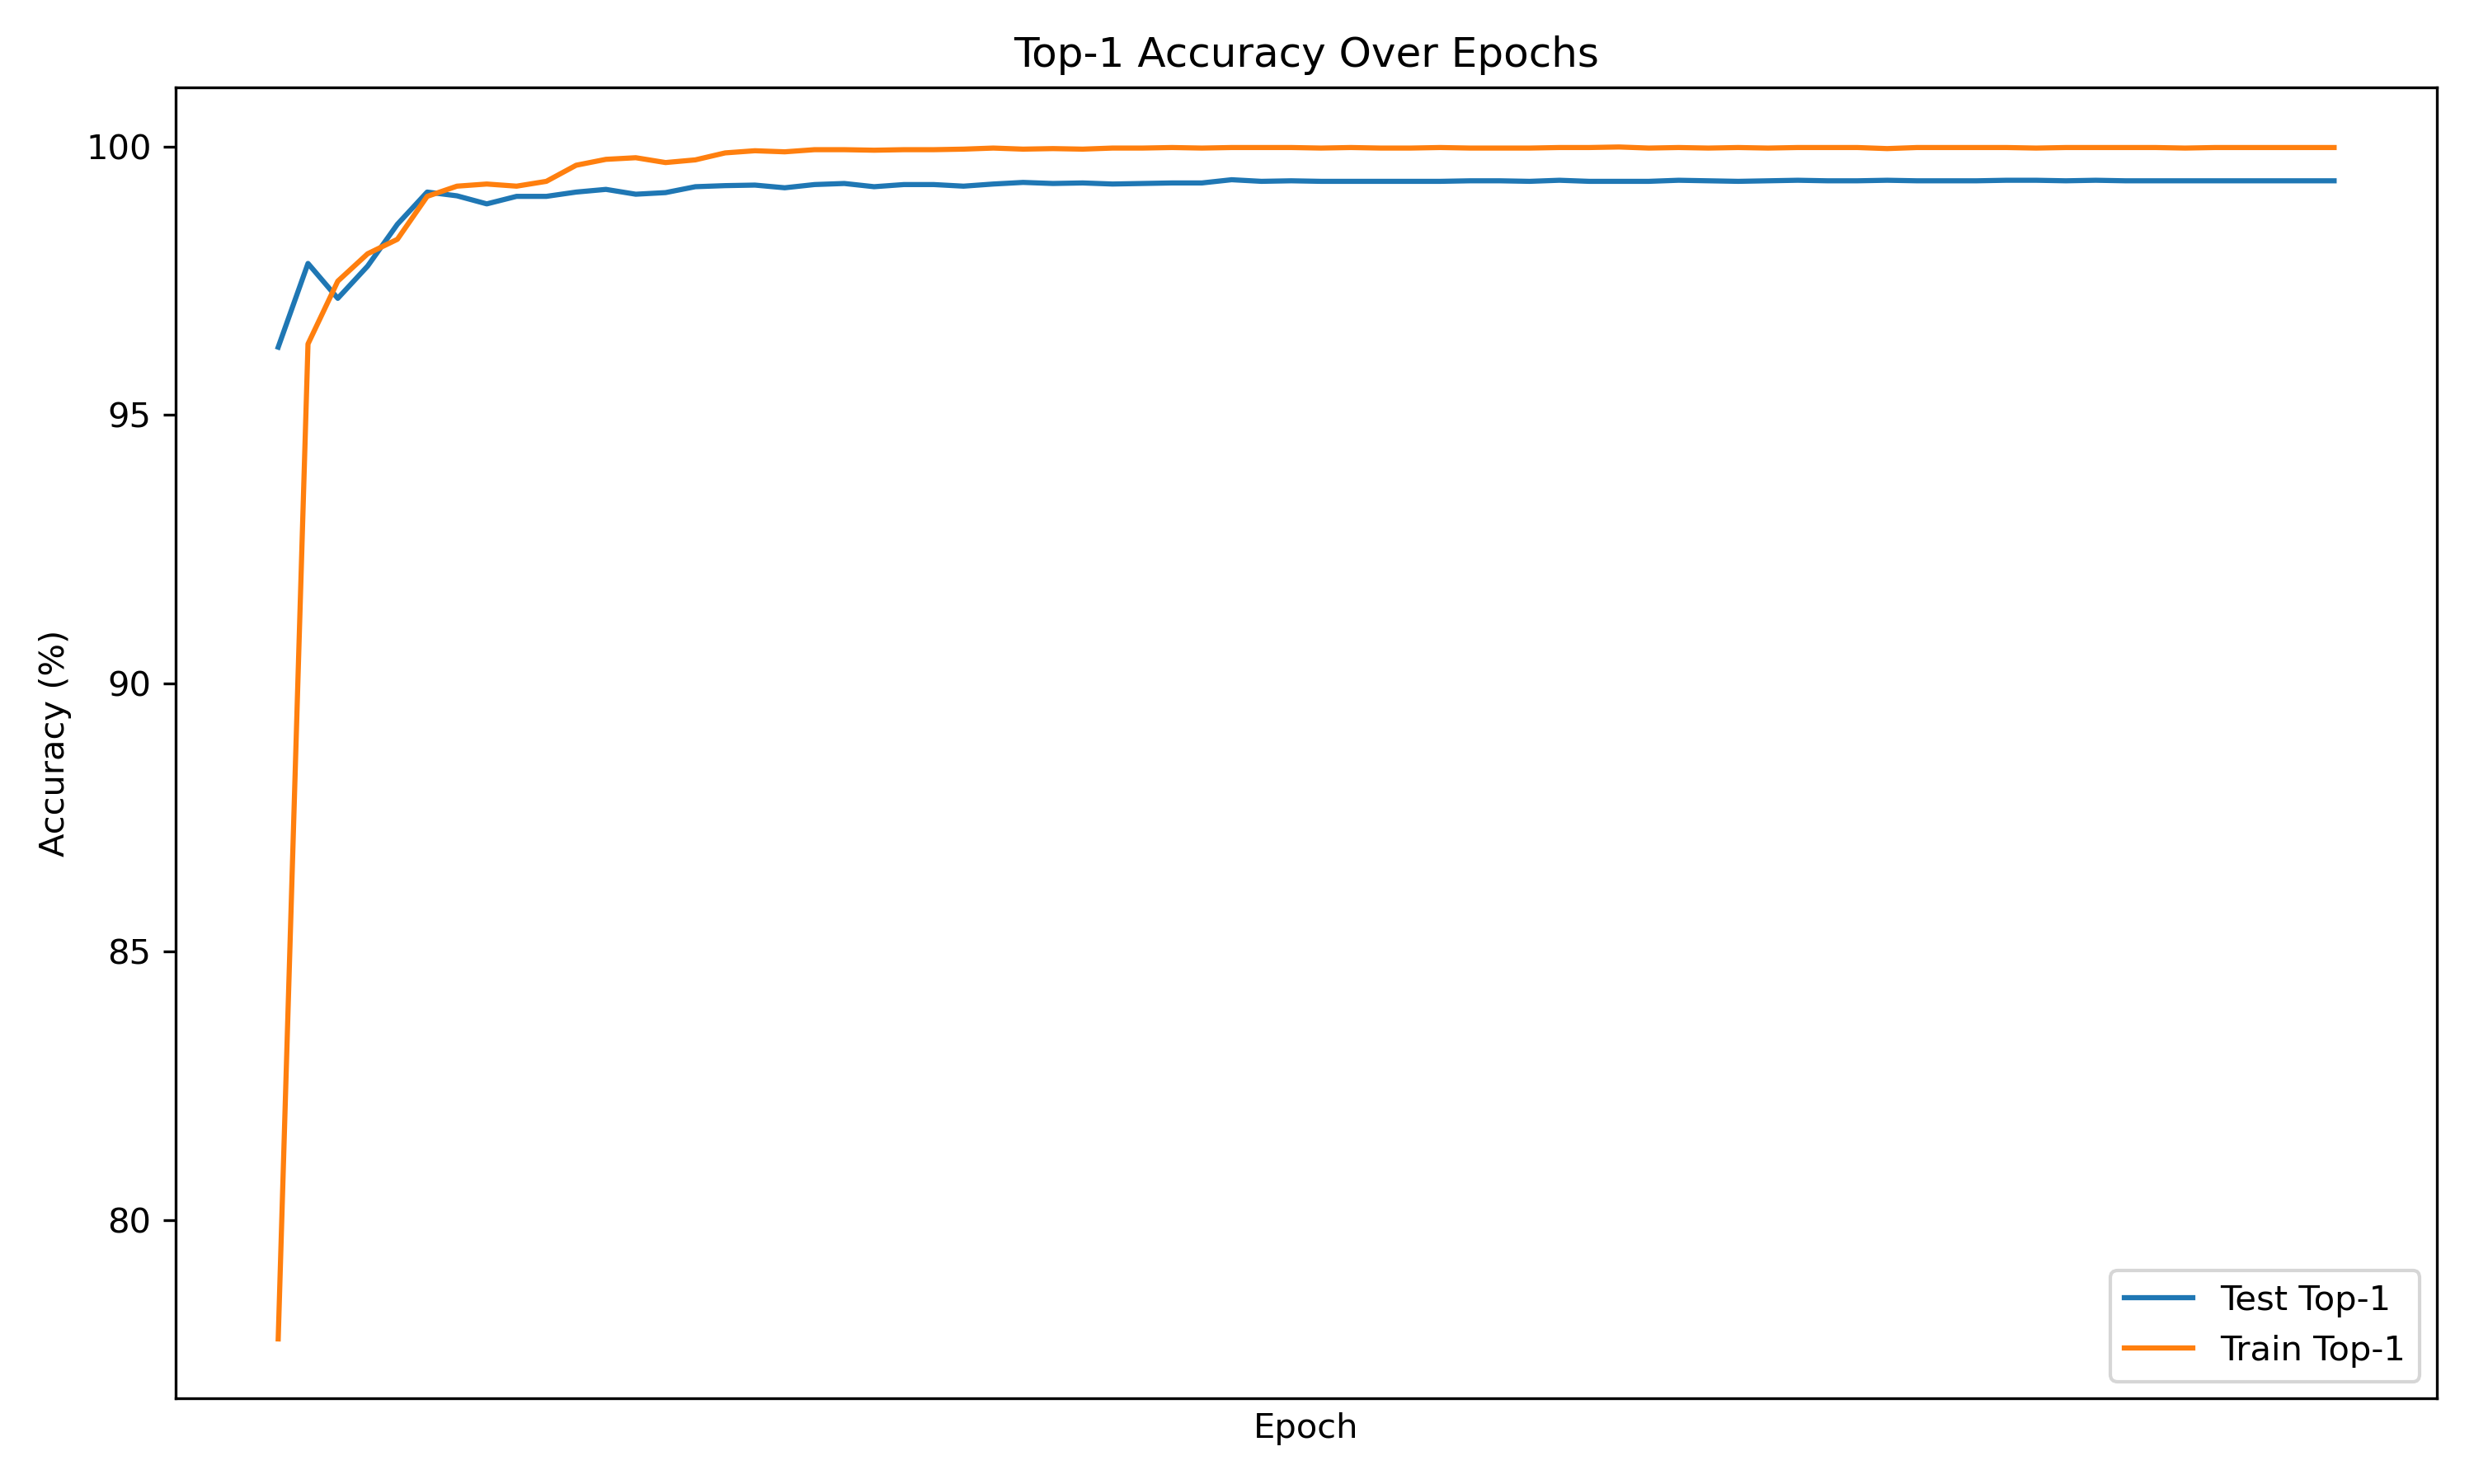
\includegraphics[width=0.85\textwidth]{transformer_images/results/mnist_original.png}
	\caption{روند دقت \lr{Top-1} مدل اصلی \lr{Swin-Tiny} بر روی \lr{MNIST}.}
	\label{fig:mnist_swin_original}
\end{figure}

\begin{figure}[ht]
	\centering
	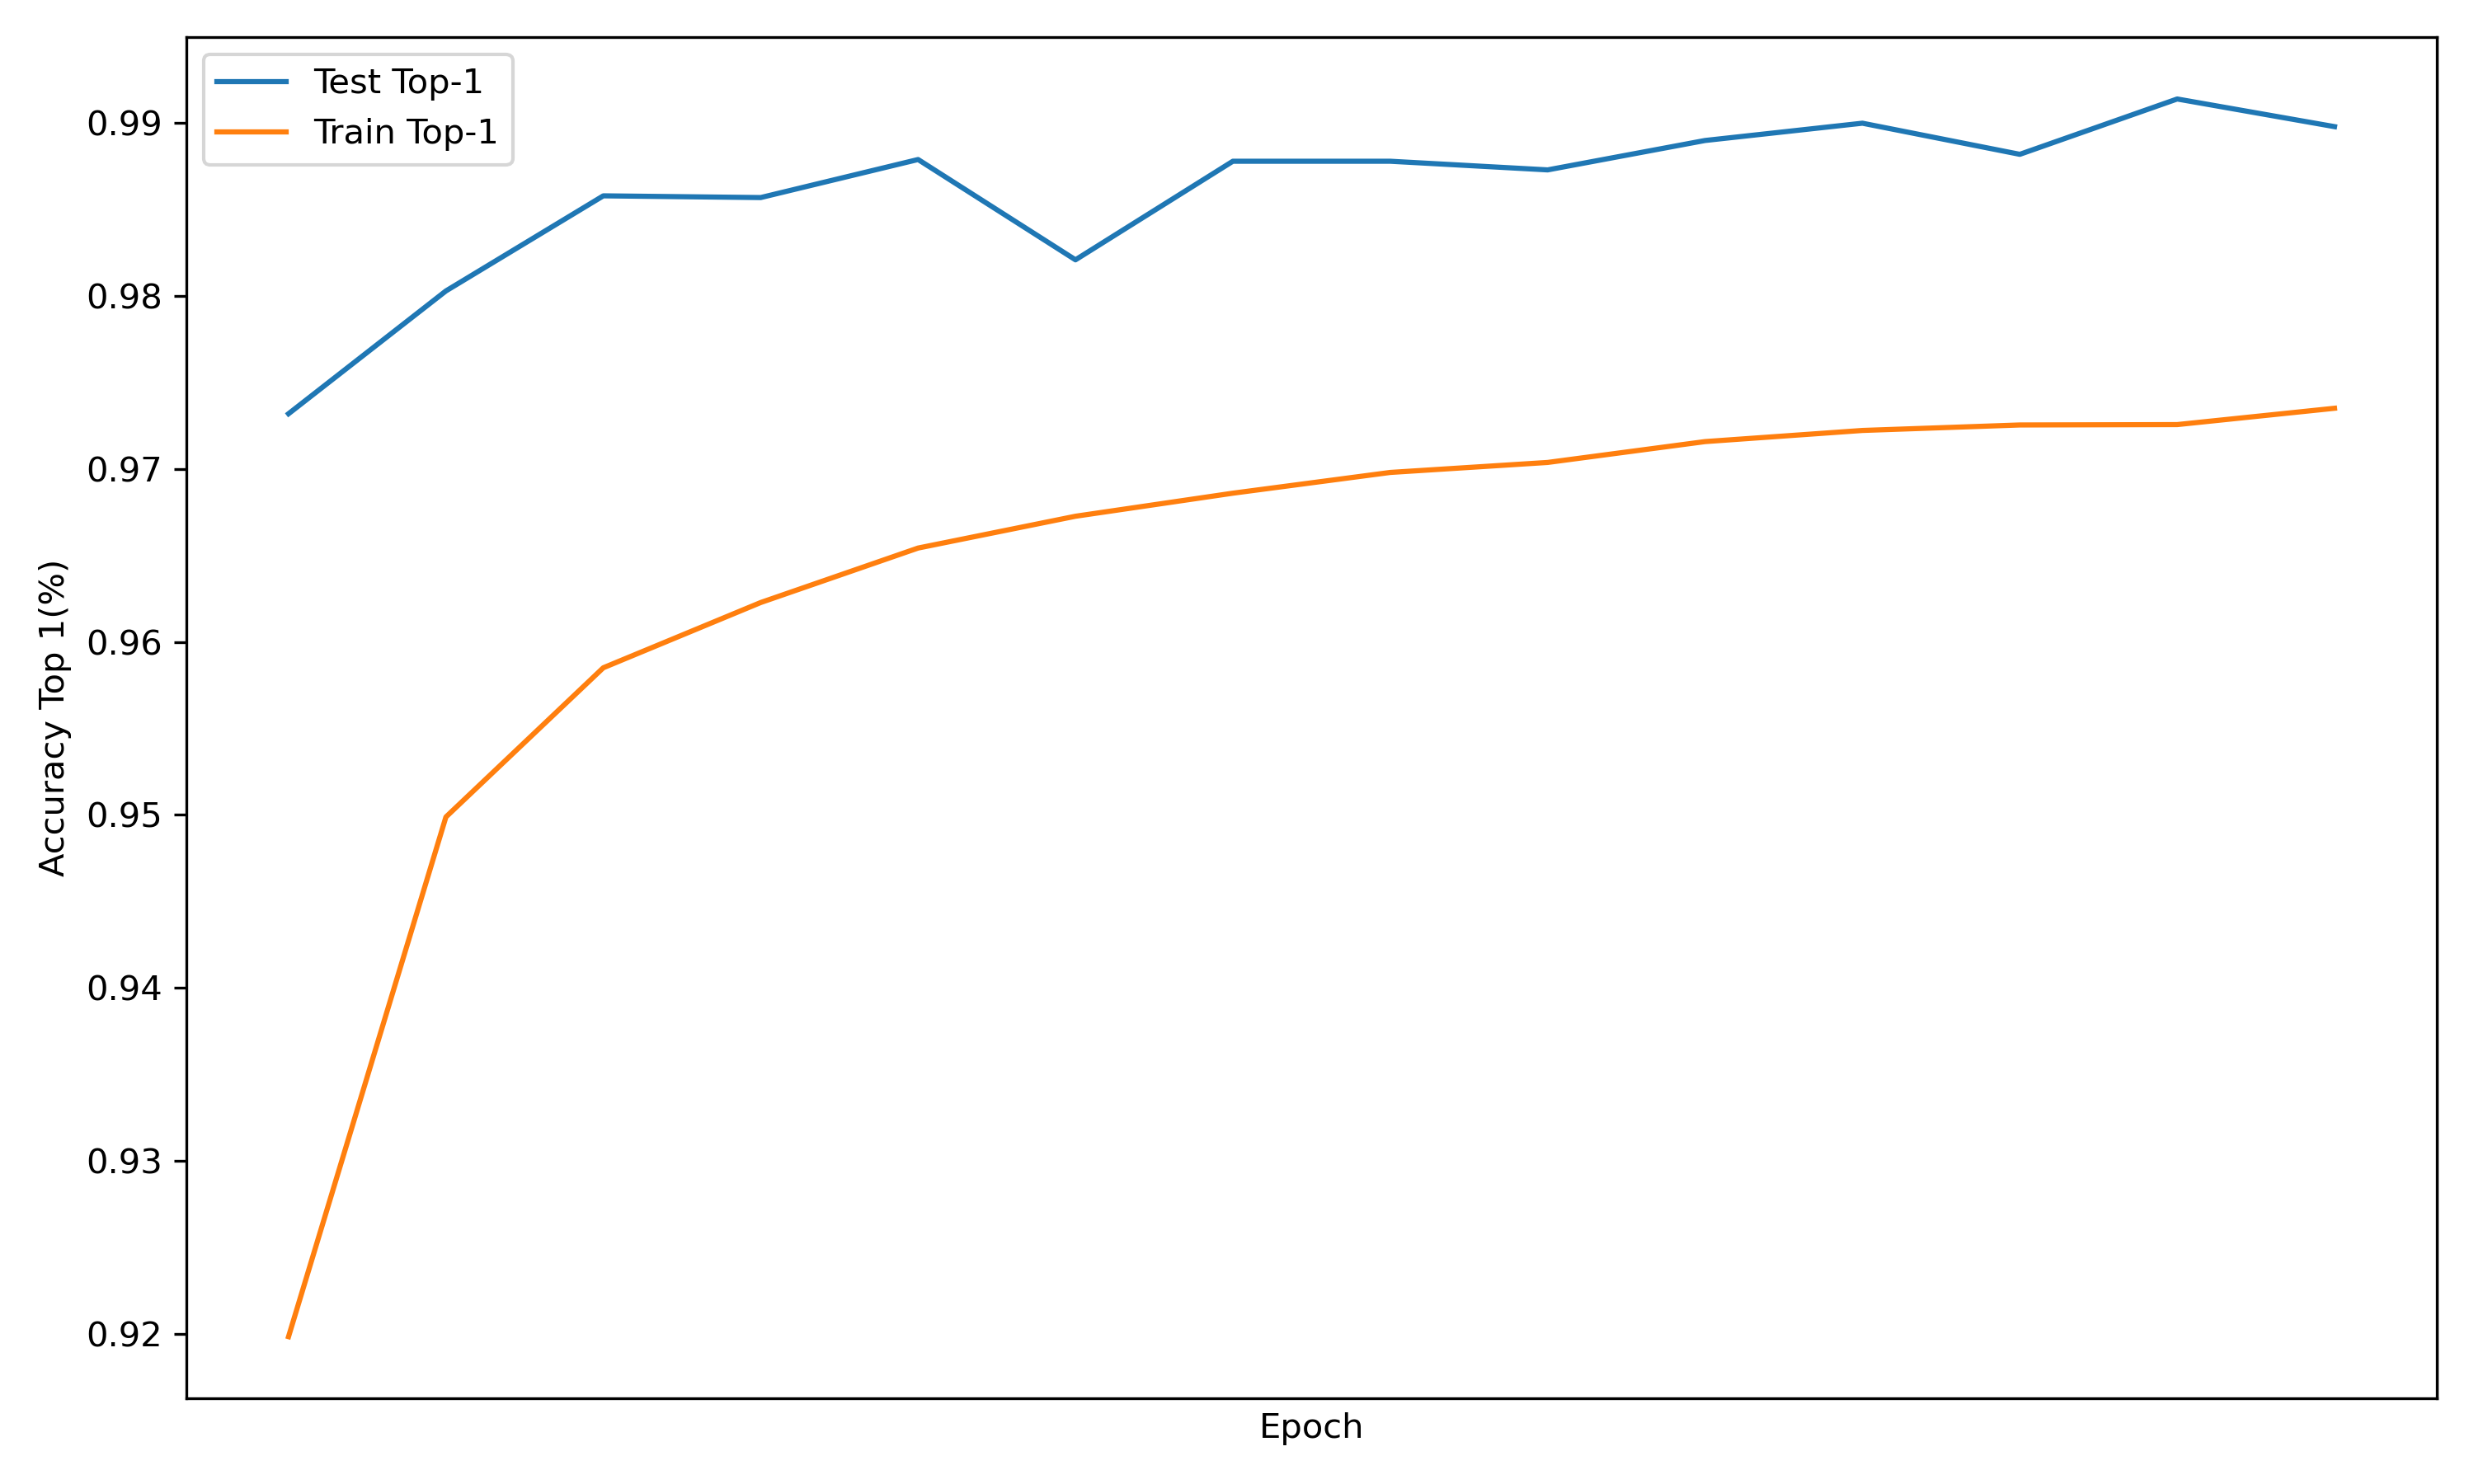
\includegraphics[width=0.85\textwidth]{transformer_images/results/mnist_tensorized.png}
	\caption{روند دقت \lr{Top-1} مدل تانسوری پیشنهادی بر روی \lr{MNIST}.}
	\label{fig:mnist_tensorized}
\end{figure}

\subsection{تحلیل و بحث}

نتایج جدول \ref{tab:mnist_summary_tensor} نشان‌دهنده‌ی نکات مهم زیر است:
\begin{itemize}
	\item \textbf{کاهش چشمگیر پارامترها:} مدل تانسوری فقط \lr{1,368,626} پارامتر دارد در حالی‌که مدل اصلی \lr{27,528,690} پارامتر دارد؛ یعنی کاهش حدوداً \textbf{\lr{20.1} برابر} (نزدیک به \textbf{\lr{95\%}} کاهش در تعداد پارامترها).
	\item \textbf{بهبود دقت آزمون:} دقت \lr{Top-1} آزمون از \textbf{\lr{97.0\%}} در مدل اصلی به \textbf{\lr{98.9\%}} در مدل تانسوری رسیده است (بهبود مطلق \textbf{\lr{+1.9}} واحد درصد). همچنین دقت \lr{Top-5} از \textbf{\lr{99.9\%}} به \textbf{\lr{100\%}} افزایش یافته است.
	\item \textbf{کاهش شکاف آموزش–آزمون:} در مدل اصلی شکاف بین آموزش و آزمون برای \lr{Top-1} برابر \textbf{\lr{1.2}} واحد درصد است (95.8 در برابر 97.0). در مدل تانسوری این شکاف به \textbf{\lr{-1.6}} واحد درصد رسیده است که نشان‌دهنده‌ی عملکرد پایدارتر و تعمیم‌پذیری بهتر است.
	\item \textbf{پایداری در داده‌های ساده‌تر:} با وجود سادگی مجموعه‌داده‌ی \lr{MNIST}، مدل تانسوری همچنان توانسته است دقت را نسبت به مدل اصلی بهبود دهد، که بیانگر قدرت فشرده‌سازی تانسوری در حفظ یا حتی افزایش دقت در کنار کاهش منابع محاسباتی است.
\end{itemize}

\paragraph{جمع‌بندی.} بر اساس نتایج به‌دست‌آمده، مدل تانسوری نه‌تنها حجم مدل را به‌شدت کاهش داده است، بلکه توانسته در یک مجموعه‌داده‌ی ساده مانند \lr{MNIST}، دقت آزمون را نسبت به مدل اصلی افزایش دهد. این نتایج مؤید این است که فشرده‌سازی تانسوری می‌تواند حتی در شرایطی که داده‌ها ساده هستند نیز به‌عنوان یک رویکرد بهینه و کارا مورد استفاده قرار گیرد.








